\documentclass[12pt, letterpaper]{article}

\usepackage{amsmath}
\usepackage[a4paper, portrait, margin=1in]{geometry}
\usepackage{hyperref}
\usepackage{minted}
\usepackage{mdframed}
\usepackage{tikz}
\usepackage{listings}
\usepackage{multirow}
\usepackage{bookmark}
\usepackage{xcolor}
\usepackage{colortbl}
\usepackage{framed}

\definecolor{shadecolor}{RGB}{240,240,240}
\newcommand{\mybox}[1]{\par\noindent\colorbox{shadecolor}
{\parbox{\dimexpr\textwidth-2\fboxsep\relax}{#1}}}

\renewcommand{\thesection}{Question \arabic{section}}
\renewcommand{\thesubsection}{\arabic{section}\alph{subsection})}
\renewcommand{\thesubsubsection}{\roman{subsubsection})}
\renewcommand{\thefigure}{\arabic{figure}}

\lstset{
basicstyle=\small\ttfamily,
columns=flexible,
breaklines=true
}

\hypersetup{
    colorlinks=true,
    linkcolor=blue,
    filecolor=magenta,      
    urlcolor=blue,
}

\setlength{\parindent}{0em}
\setlength{\parskip}{1em}


\title{CSS601 Introduction to Artificial Intelligence - Assignment 2}
\author{Ian Chong Wei Ming\\
\href{mailto:ian.chong.2020@mitb.smu.edu.sg}{ian.chong.2020@mitb.smu.edu.sg}\\
+65-9680-8118}
\date{\today}

\begin{document}

\maketitle

\mybox{\textbf{Note:} Given information will be shaded \underline{grey} or in \textit{tables}.}

\section{Heuristic Search}
\begin{center}
    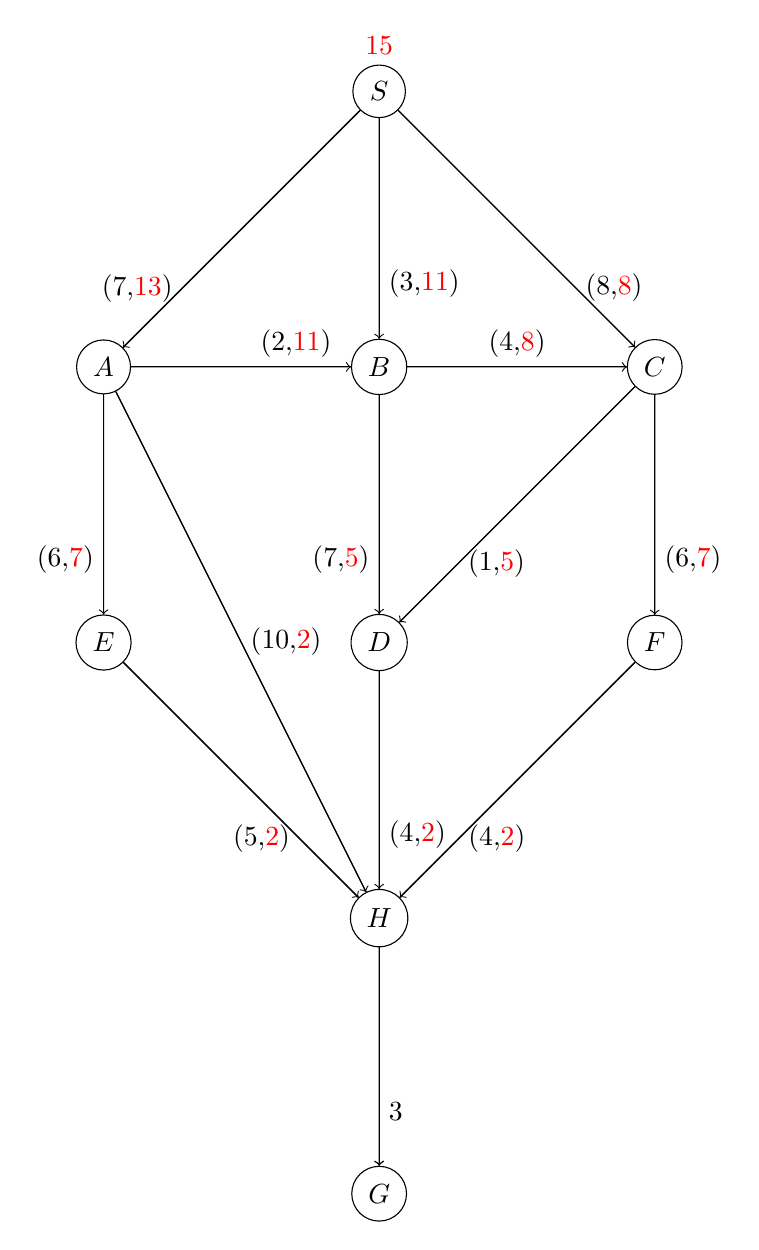
\begin{tikzpicture}[node distance=3.5cm]
        
        \node[circle,draw,label={\textcolor{red}{15}}] (S) {$S$};
        \node[circle,draw, below of=S] (B) {$B$};
        \node[circle,draw, left of=B] (A) {$A$};
        \node[circle,draw, right of=B] (C) {$C$};
        \node[circle,draw, below of=B] (D) {$D$};
        \node[circle,draw, below of=A] (E) {$E$};
        \node[circle,draw, below of=C] (F) {$F$};
        \node[circle,draw, below of=D] (H) {$H$};
        \node[circle,draw, below of=H] (G) {$G$};
    
        \path [->,draw] 
        (S) -- (B)
        (S) -- (A)
        (S) -- (C)
        (A) -- (B)
        (A) -- (E)
        (A) -- (H)
        (B) -- (C)
        (B) -- (D)
        (C) -- (D)
        (C) -- (F)
        (E) -- (H)
        (D) -- (H)
        (F) -- (H)
        (H) -- (G);
    
        \path[->,draw]
        (S) edge node[right, near end] {(3,\textcolor{red}{11})} (B)
        (S) edge node[left, near end] {(7,\textcolor{red}{13})} (A)
        (S) edge node[right, near end] {(8,\textcolor{red}{8})} (C)
        (A) edge node[above, near end] {(2,\textcolor{red}{11})} (B)
        (A) edge node[left, near end] {(6,\textcolor{red}{7})} (E)
        (A) edge node[right] {(10,\textcolor{red}{2})} (H)
        (B) edge node[above] {(4,\textcolor{red}{8})} (C)
        (B) edge node[left, near end] {(7,\textcolor{red}{5})} (D)
        (C) edge node[right, near end] {(1,\textcolor{red}{5})} (D)
        (C) edge node[right, near end] {(6,\textcolor{red}{7})} (F)
        (E) edge node[left, near end] {(5,\textcolor{red}{2})} (H)
        (D) edge node[right, near end] {(4,\textcolor{red}{2})} (H)
        (F) edge node[right, near end] {(4,\textcolor{red}{2})} (H)
        (H) edge node[right, near end] {3} (G);
    \end{tikzpicture}
\end{center}

\mybox{For the above graph (heuristic values are provided in red color and actual costs are in black
color), please provide answers to the following answers. Also note that S is start state and G
is goal state.}

\subsubsection{Is the heuristic admissible?}

\textbf{Response:} A heuristic is defined as \textit{admissible} if it never \textit{overestimates} the \textbf{cost} of reaching the \textbf{goal}. 
In otherwords, the cost that estimated by the heuristic to reach the goal \textbf{cannot} be \textit{higher} than the \textit{lowest} possible cost from the \textit{current point} in the path.
More formally, $h(n)\leq c(n,g) \forall n$

The minimum cost and the heuristic $h(n)$ to reach the goal from each node is given in the following table.
Workings will follow the table.

\begin{center}
    \begin{tabular}{|c|c|c|c|} 
    \hline
    Node $n$ & $c(n,g)$ & $h(n)$ & $h(n)\leq c(n,g)?$ \\ 
    \hline
    S & 15 & 15 & TRUE\\
    \hline
    A & 13 & 13 & TRUE\\
    \hline
    B & 12 & 11 & TRUE\\
    \hline
    C & 8 & 8 & TRUE\\
    \hline
    E & 8 & 7 & TRUE\\
    \hline
    D & 7 & 5 & TRUE\\
    \hline
    F & 7 & 7 & TRUE\\
    \hline
    H & 3 & 2 & TRUE\\
    \hline
    \end{tabular}
\end{center}

\textbf{Node S}

The path to follow would be $S\rightarrow B\rightarrow C\rightarrow D\rightarrow H\rightarrow G$

$c(n,g)=3+4+1+4+3=\underline{\textbf{15}}$

$h(n)=\textcolor{red}{15}$

\textbf{Node A}

The path to follow would be $A\rightarrow H\rightarrow G$

$c(n,g)=\underline{\textbf{13}}$

$h(n)=\textcolor{red}{13}$

\textbf{Node B}

The path to follow would be $B\rightarrow C\rightarrow D\rightarrow H\rightarrow G$

$c(n,g)=4+4+1+3=\textbf{\underline{12}}$

$h(n)=\textcolor{red}{11}$

\textbf{Node C}

The path to follow would be $C\rightarrow D\rightarrow H\rightarrow G$

$c(n,g)=1+4+3=\underline{\textbf{8}}$

$h(n)=\textcolor{red}{8}$

\textbf{Node D}

The path to follow would be $D\rightarrow H\rightarrow G$

$c(n,g)=4+3=\underline{\textbf{7}}$ 

$h(n)=\textcolor{red}{5}$

\textbf{Node E}

The path to follow would be $E\rightarrow H\rightarrow G$

$c(n,g)=5+3=\underline{\textbf{8}}$ 

$h(n)=\textcolor{red}{7}$

\textbf{Node F}

The path to follow would be $F\rightarrow H\rightarrow G$

$c(n,g)=4+3=\underline{\textbf{7}}$ 

$h(n)=\textcolor{red}{7}$

\textbf{Node H}

The path to follow would be $H\rightarrow G$

$c(n,g)=\underline{\textbf{3}}$ 

$h(n)=\textcolor{red}{2}$

Since $h(n)\leq c(n,g) \forall n$, the heuristic is \textit{admissible}.

\subsubsection{Is the heuristic consistent? Provide justification}
\textbf{Response:} No, the heuristic is not \textit{consistent}.

A heuristic is \textit{consistent} only if 

a) It is \textit{admissible} and;

b) Its estimate is \underline{always} less than or equal to the estimated distance from any neighbouring vertex to the goal, plus the cost of reaching that neighbour. More formally:

\[h(n) \leq c(n,p) + h(p) \forall n\]

Non-consistent nodes in the following table are coloured \colorbox{red}{RED}

\begin{center}
    \begin{tabular}{|c|c|c|c|} 
    \hline
    Node $n$ & $h(n)$ & $p$ & $c(n,p)+h(p)$ \tabularnewline
    \hline
    S & 15 & A & 20\tabularnewline
    \hline
    \rowcolor{red}S & 15 & B & 14\tabularnewline
    \hline
    S & 15 & C & 16\tabularnewline
    \hline
    A & 13 & B & 13\tabularnewline
    \hline
    A & 13 & E & 13\tabularnewline
    \hline
    \rowcolor{red}A & 13 & H & 12\tabularnewline
    \hline
    B & 11 & C & 12\tabularnewline
    \hline
    B & 11 & D & 12\tabularnewline
    \hline
    \rowcolor{red}C & 8 & D & 6\tabularnewline
    \hline
    C & 8 & F & 13\tabularnewline
    \hline
    D & 5 & H & 6\tabularnewline
    \hline
    E & 7 & H & 7\tabularnewline
    \hline
    \rowcolor{red}F & 7 & H & 6\tabularnewline
    \hline
    H & 2 & G & 3\tabularnewline
    \hline

    \end{tabular}
\end{center}

\subsubsection{DFS, BFS, Best First Search and A* Search}
\mybox{Provide the search steps (as discussed in class) with DFS, BFS (with and without priority
queue), Best First Search and A* search. Specify for each algorithm if the open list is
queue, stack, or priority queue. Feel free to add rows/columns, or other details in the
table below. Open list contains nodes that are to be explored, and “Nodes to add” are
the successors of the node that is recently popped.}

\textbf{Response:} The following tables detail the steps each algorithm takes.

\begin{center}
    \begin{tabular}{|c|c|c|c|}
    \hline
    \multicolumn{4}{|c|}{Depth First Search (\textbf{DFS})\textcolor{red}{*}}\\
    \hline
    Step No. & Open List & POP & Nodes to add \\ 
    \hline
    1 & $S$ & $S$ & $A^S, B^S, C^S$ \\
    \hline
    2 & $A^S, B^S, C^S$ & $A^S$ & $E^A,H^A$ \\
    \hline
    3 & $E^A, H^A, B^S, C^S$ & $E^A$ & nil \\
    \hline
    4 & $H^A, B^S, C^S$ & $H^A$ & $G^H$ \\
    \hline
    5 & $G^H,B^S,C^S$ & $G^H$ & nil \\
    \hline
    \end{tabular}
\end{center}

\textcolor{red}{*Open List is a \textit{stack}}

The path to follow is $S\rightarrow A\rightarrow H\rightarrow G$

Cost = 7 + 10 + 3 = \underline{\textbf{20}}

\begin{center}
    \begin{tabular}{|c|c|c|c|}
    \hline
    \multicolumn{4}{|c|}{Breadth First Search (\textbf{BFS})}\\
    \hline
    Step No. & Open List\textcolor{red}{*} & POP & Nodes to add \\ 
    \hline
    1 & $S$ & $S$ & $A^S, B^S, C^S$ \\
    \hline
    2 & $A^S, B^S, C^S$ & $A^S$ & $E^A,H^A$ \\
    \hline
    3 & $B^S, C^S, E^A, H^A$ & $B^S$ & $D^B$ \\
    \hline
    4 & $C^S, E^A, H^A, D^B$ & $C^S$ & $F^C$ \\
    \hline
    5 & $E^A,H^A,D^B,F^C$ & $E^A$ & nil \\
    \hline
    6 & $H^A,D^B,F^C$ & $H^A$  & $G^H$ \\
    \hline
    7 & $D^B,F^C,G^H$ & $D^B$  & nil \\
    \hline
    8 & $F^C,G^H$ & $F^C$  & nil \\
    \hline
    9 & $G^H$ & $G^H$  & nil \\
    \hline
    \end{tabular}
\end{center}

\textcolor{red}{*Open List is a \textit{queue}}

The path to follow is $S\rightarrow A\rightarrow H\rightarrow G$

Cost = 7 + 10 + 3 = \underline{\textbf{20}}

\begin{center}
    \begin{tabular}{|c|c|c|c|}
    \hline
    \multicolumn{4}{|c|}{Breadth First Search (\textbf{BFS} - Optimal)}\\
    \hline
    Step No. & Open List\textcolor{red}{*} & POP & Nodes to add \\ 
    \hline
    1 & $S$ & $S$ & $B^{S,3}, A^{S,7}, C^{S,8}$\\
    \hline
    2 & $B^{S,3}, A^{S,7}, C^{S,8}$ & $B^{S,3}$ & $C^{B,7},D^{B,10}$ \\
    \hline
    3 & $A^{S,7}, C^{B,7}, D^{B,10}$ & $A^{S,7}$ & $E^{A,13}, H^{A,17}$ \\
    \hline
    4 & $C^{B,7}, D^{B,10}, E^{A,13}, H^{A,17}$ & $C^{B,7}$ & $D^{C,8}, F^{C,13}$\\
    \hline
    5 & $D^{C,8}, E^{A,13}, F^{C,13}, H^{A,17}$ & $D^{C,8}$ & $H^{D,12}$\\
    \hline
    6 & $H^{D,12}, E^{A,13}, F^{C,13}$ & $H^{D,12}$ & $G^{H,15}$\\
    \hline
    7 & $E^{A,13}, F^{C,13}, G^{H,15}$ & $E^{A,13}$ & $H^{E,18}$\textcolor{red}{**}\\
    \hline
    8 & $F^{C,13}, G^{H,15}$ & $F^{C,13}$ & $H^{F,18}$\textcolor{red}{**}\\
    \hline
    9 & $G^{H,15}$ & $G^{H,15}$ & nil\\
    \hline
    \end{tabular}
\end{center}

\textcolor{red}{*Open List is a \textit{priority queue}}

\textcolor{red}{**not added to the Open list since it is already \textit{explored}}

The path to follow is $S\rightarrow B\rightarrow C\rightarrow D\rightarrow H\rightarrow G$

Cost = 3 + 4 + 1 + 4 + 3 = \underline{\textbf{15}}

\begin{center}
    \begin{tabular}{|c|c|c|c|}
    \hline
    \multicolumn{4}{|c|}{Best First Search}\\
    \hline
    Step No. & Open List\textcolor{red}{*} & POP & Nodes to add \\ 
    \hline
    1 & $S$ & $S$ & $A^{S,13}, B^{S,11}, C^{S,8}$ \\
    \hline
    2 & $C^{S,8}, B^{S,11}, A^{S,13}$ & $C^{S,8}$ & $D^{C,5}, F^{C,7}$ \\
    \hline
    3 & $D^{C,5}, F^{C,7}, B^{S,11}, A^{S,13}$ & $D^{C,5}$ & $H^{D,2}$ \\
    \hline
    4 & $H^{D,2}, F^{C,7}, B^{S,11}, A^{S,13}$ & $H^{D,2}$ & $G^{H,0}$\\
    \hline
    5 & $G^{H,0}, F^{C,7}, B^{S,11}, A^{S,13}$ & $G^{H,0}$ & nil\\
    \hline
    \end{tabular}
\end{center}

\textcolor{red}{*Open List is a \textit{priority queue}}

The path to follow is $S\rightarrow C\rightarrow D\rightarrow H\rightarrow G$

Cost = 8 + 1 + 4 + 3 = \underline{\textbf{16}}

\begin{center}
    \begin{tabular}{|c|c|c|c|}
    \hline
    \multicolumn{4}{|c|}{A* Search}\\
    \hline
    Step No. & Open List\textcolor{red}{*} & POP & Nodes to add \\ 
    \hline
    1 & $S$ & $S^{15}$ & $B^{S,14}, C^{S,16}, A^{S,20}$ \\
    \hline
    2 & $B^{S,14}, C^{S,16}, A^{S,20}$ & $B^{S,14}$ & $C^{B,15}, D^{B,15}$ \\
    \hline
    3 & $C^{B,15}, D^{B,15}, A^{S,20}$ & $C^{B,15}$ & $D^{C,13},F^{C,20}$ \\
    \hline
    4 & $D^{C,13}, A^{S,20}, F^{C,20}$ & $D^{C,13}$ & $H^{D,14}$\\
    \hline
    5 & $H^{D,14}, A^{S,20}, F^{C,20}$ & $H^{D,14}$ & $G^{H,15}$\\
    \hline
    6 & $G^{H,15}, A^{S,20}, F^{C,20}$ & $G^{H,15}$ & nil\\
    \hline
    \end{tabular}
\end{center}

\textcolor{red}{*Open List is a \textit{priority queue}}

The path to follow is $S\rightarrow B\rightarrow C\rightarrow D\rightarrow H\rightarrow G$

Cost = 3 + 4 + 1 + 4 + 3 = \underline{\textbf{15}}

\section{Build an automated car in a simulator}

\mybox{The goal of this assignment is to guide your car to move in a multi-lane straight road (represented using a rectangular grid) simulator (details explained later). 

In addition to your car, there are other cars also moving along the road. You need to design an algorithm which can take your car from its start position to the end of the road as soon as possible while avoiding other cars. 

Other cars are moving randomly. At any step, your car can view up to 4 cells in front, left and right, i.e., it will not be able to look at the other cars which are beyond its visibility range of 4 cells. (This visibility range of 4 is configurable and your algorithm should work irrespective of visibility range).

We describe the state, operators and goal state for this problem below.

\textbf{State}: State of the car is its location, i.e., the grid cell it is currently present in. 

\textbf{Operators/Actions}: Following are the available operators or actions for the car:

\begin{itemize}
    \item \textbf{Forward} – Moves the car one step ahead in the same lane.
    \item \textbf{Forward-2$\times$} – Moves the car two steps ahead in the same lane.
    \item \textbf{Forward-3$\times$} – Moves the car three steps ahead in the same lane.
    \item \textbf{Left} – Moves the car in the left lane and one step forward.
    \item \textbf{Right} – Moves the car in the right lane and one step forward.
    \item \textbf{None} – Stays at the same place.
\end{itemize}

If the action is unsuccessful then the car will stay at the same place. Action will be unsuccessful if there is a wall or another car present in the intended direction of move. For example, a forward will be unsuccessful if there is another car present in front of your car.
As the left action moves a car to the left and one step forward, a left action taken in grid cell (5,3) will be unsuccessful if there is a car in either of (4,3) or (4,4).

\textbf{Goal State:} There is one goal state, where your car needs to reach.}

\subsection{Write the function}
\mybox{Write the function that will generate the \textbf{operator/action} to be taken at the current time step (based on search algorithms discussed in class), so that time taken to reach goal is as \textit{minimal} as possible. 
[You may refer to “\texttt{pseudo code.pdf}” for implementation details and pseudo code for $A* Search$.]
The code for the Simulator is provided in the zip file \texttt{"SelfDrivingCar.zip"}. The details about the
installation/running of simulator and code details are provided in the file \texttt{"SelfDrivingCar.pdf"}
(present in the \texttt{.zip} file).}

\textbf{Response:} Please see attached \texttt{python} script.

\subsection{Submit code in \texttt{.pdf}}

\textbf{Response:}

\subsubsection{Algorithm 1 - \texttt{drive}}

This is the code for the main drive code. It depends on the subsequent helper functions.

\begin{mdframed}[backgroundcolor=shadecolor]
\begin{minted}[fontsize=\footnotesize,breaklines]{python}
def drive(self, goalstates, inputs):    
    
    path_list = []
    destination_reached = []
    action_order = []
    path_lengths = []
    start = self.state

    for goal in goalstates:
        goalReached, path = self.AStar(start["location"], goal, inputs)
        destination_reached.append(goalReached)
        path_list.append(path)
        path_lengths.append(len(path))
    
    if True in destination_reached:        
        best_path = [path_list[i] for i in range(len(path_list)) if (destination_reached[i] == True) and (len(path_list[i]) == min(path_lengths))]
        action_order.extend(best_path)
    else:        
        longest_path = [path_list[i] for i in range(len(path_list)) if (len(path_list[i]) == max(path_lengths))]
        action_order.extend(longest_path)

    movements = {
        (0, 3): "forward-3x", 
        (0, 2): "forward-2x", 
        (0, 1): "forward", 
        (-1, 1): "left", 
        (1, 1): "right", 
        (0, 0): None}
    try:
        action_sequence = [movements[(action_order[0][i+1][0] - action_order[0][i][0], action_order[0][i+1][1] - action_order[0][i][1])] for i in range(len(action_order[0])-1)]
    except:
        action_sequence = [None]
    
    return action_sequence
\end{minted}
\end{mdframed}

\subsubsection{Algorithm 2 - \texttt{AStar}}

Implementation of $A* Search$ to car to consider which action to take. Relies on \texttt{applyAction} to function properly.

\begin{mdframed}[backgroundcolor=shadecolor]
\begin{minted}[fontsize=\footnotesize,breaklines]{python}
def AStar(self, start, goal, state):    
    closedSet = []
    openSet = [start]
    cameFrom = {}
    gScore = {start: 0}
    fScore = {start: self.heuristic_cost_estimate(start, goal)}
    current = []
    
    while len(openSet) > 0:
        min_idx = list(fScore.values()).index(min(fScore.values()))
        current = list(fScore.keys())[min_idx]
        if current == goal["location"]:
            return True, self.reconstruct_path(cameFrom, current)
        del fScore[current]
        openSet.remove(current)
        closedSet.append(current)
        
        for action in ["forward-3x", "forward-2x", "forward", "left", "right"]:
            neighbor = self.applyAction(current, action, state, goal["location"])
            if neighbor == current:
                continue
            tentative_gScore = gScore[current] + 1
            if neighbor not in openSet:
                openSet.append(neighbor)
            elif tentative_gScore >= gScore[neighbor]:
                continue
            cameFrom[neighbor] = current
            gScore[neighbor] = tentative_gScore
            fScore[neighbor] = gScore[neighbor] + self.heuristic_cost_estimate(neighbor, goal)
        
    if current == goal["location"]:
        return True, self.reconstruct_path(cameFrom, current)
    else:
        return False, self.reconstruct_path(cameFrom, current)
\end{minted}
\end{mdframed}

\subsubsection{Algorithm 2.5 - \texttt{applyAction}}

Helper function to determine if a move is valid and apply it. For invalid moves, returns the current position \textit{i.e.} no action

\begin{mdframed}[backgroundcolor=shadecolor]
\begin{minted}[fontsize=\footnotesize,breaklines]{python}
def applyAction(self, current, action, state, goal):
    movements = {
        "forward-3x": [(0, 1), (0, 2), (0, 3)], 
        "forward-2x": [(0, 1), (0, 2)], 
        "forward": [(0, 1)], 
        "left": [(-1, 0), (-1, 1)], 
        "right": [(1, 0), (1, 1)], 
        None: [(0, 0)]}
    
    target_row = current[0]
    target_col = current[1]
    valid_move = True
    
    for movement in movements[action]:
        if (target_row + movement[0] >= len(state)) or \
            (target_row + movement[0] < 0) or \
            (target_col + movement[1]) >= len(state[0]):
            return current
                
        if state[target_row + movement[0]][target_col + movement[1]] == 1:
            valid_move = False
            break
        
    if abs(target_row + movements[action][-1][0] - goal[0]) > abs(goal[1] - (target_col + movements[action][-1][1])):
        return current
    
    if valid_move:
        target_row += movements[action][-1][0]
        target_col += movements[action][-1][1]
    return (target_row, target_col)
\end{minted}
\end{mdframed}

\subsubsection{Algorithm 3 - \texttt{heuristic\_cost\_estimate}}

Estimates the heuristic cost from current node.

\begin{mdframed}[backgroundcolor=shadecolor]
\begin{minted}[fontsize=\footnotesize,breaklines]{python}
def heuristic_cost_estimate(self, start, goal):
    result = abs(goal["location"][1] - start[1]) + abs(goal["location"][0] - start[0]) / 2
    return result
\end{minted}
\end{mdframed}

\subsubsection{Algorithm 4 - \texttt{reconstruct\_path}}

Helper function to reconstruct the path from start to current node.

\begin{mdframed}[backgroundcolor=shadecolor]
\begin{minted}[fontsize=\footnotesize,breaklines]{python}
def reconstruct_path(self, cameFrom, current):
    total_path = []
    while current in cameFrom.keys():
        total_path.append(current)
        current = cameFrom[current]
    total_path.append(current)
    total_path = total_path[::-1]
    return total_path
\end{minted}
\end{mdframed}

\section{Taxi Driver Markov Decision Process}
\mybox{Taxi drivers in Singapore can pick up customers from any location that is not on highways. 
However, they require guidance on where to pick up customers when they do not have customers on board and there are no bookings. 
In this question, we address this guidance problem. 
There are four locations: $L1$, $L2$, $L3$ and $L4$ from where taxi drivers can pick up and drop off customers. 
At any decision epoch, the chances of the taxi driver picking up a customer from different locations are provided in \textbf{Table 1} below:}

\begin{center}
    \textbf{Table 1}

    \begin{tabular}{|c|c|} 
    \hline
    Location & Chance of finding customer\\ 
    \hline
    $L1$ & 0.3 \\
    \hline
    $L2$ & 0.8 \\
    \hline
    $L3$ & 0.1 \\
    \hline
    $L4$ & 0.6 \\
    \hline
    \end{tabular}
    
\end{center}

\mybox{Once the taxi driver picks up a customer, the customer determines the destination. Observed
probabilities (from past data) of a customer starting from a source location and going to a
destination location are given below:}

\begin{center}
    \textbf{Table 2}

    \begin{tabular}{|c|c|} 
    \hline
    $Source \rightarrow Destination$ & Probability\\ 
    \hline
    $L1 \rightarrow L2$ & 0.4 \\
    \hline
    $L1 \rightarrow L3$ & 0.35 \\
    \hline
    $L1 \rightarrow L4$ & 0.25 \\
    \hline
    $L2 \rightarrow L1$ & 0.4 \\
    \hline
    $L2 \rightarrow L3$ & 0.6 \\
    \hline
    $L3 \rightarrow L1$ & 0.6 \\
    \hline
    $L3 \rightarrow L4$ & 0.4 \\
    \hline
    $L4 \rightarrow L1$ & 0.65 \\
    \hline
    $L4 \rightarrow L2$ & 0.35 \\
    \hline
    \end{tabular}    
\end{center}
\mybox{\textit{**If a source destination pair does not appear in the above table, it indicates the fare is 0.}

Cost of travelling between locations is as follows:}

\begin{center}
    \textbf{Table 3}

    \begin{tabular}{|c|c|} 
    \hline
    $Source \rightarrow Destination$ & Cost (\$)\\ 
    \hline
    $L1 \rightarrow L2$ & 1.00 \\
    \hline
    $L1 \rightarrow L3$ & 1.50 \\
    \hline
    $L1 \rightarrow L4$ & 1.25 \\
    \hline
    $L2 \rightarrow L1$ & 1.00 \\
    \hline
    $L2 \rightarrow L3$ & 0.75 \\
    \hline
    $L3 \rightarrow L1$ & 1.50 \\
    \hline
    $L3 \rightarrow L4$ & 0.80 \\
    \hline
    $L4 \rightarrow L1$ & 1.25 \\
    \hline
    $L4 \rightarrow L2$ & 1.00 \\
    \hline
    \end{tabular}
\end{center}
\textit{**If a source destination pair does not appear in the above table, it indicates the cost is infinity. If the taxi does not move (i.e., source and destination are same), then the cost is zero.}

\mybox{The taxi driver can either pickup from the current location or move to another location. 
Pickup corresponds to picking up a customer (if one is found) and dropping them of at their destination. 
Pickup action succeeds with probabilities specified in \textbf{Table 1} and if the taxi picks up a customer, destination location is determined by the probabilities in \textbf{Table 2}. 
When Pickup action fails, the taxi remains in its current location. 
Move to another location is always successful and taxi moves to the desired location with probability 1.
Both pickup and move actions take one-time step each. Please provide the following:}

\subsection{MDP Model for "move and pickup customers"}

\begin{center}
    \begin{tabular}{|c|l|c|r|r|}
    \hline
    s (current state)       &$a$ (action) & $s'$ (new state) & $P(s'|s,a)$ & $R(s,a,s')$ 
    \\ \hline
    \multirow{8}{*}{$L1$}   & Pick-up $\rightarrow$ $L1$ & $L1$ & $1-0.3=0.70$ & $0$ \\ \cline{2-5} 
                            & Pick-up $\rightarrow$ $L2$ & $L2$ & $0.3\times 0.4=0.12$ & $8-1=7$ \\ \cline{2-5} 
                            & Pick-up $\rightarrow$ $L3$ & $L3$ & $0.3\times 0.35=0.11$ & $13-1.5=11.5$ \\ \cline{2-5} 
                            & Pick-up $\rightarrow$ $L4$ & $L4$ & $0.3\times 0.25=0.075$ & $15-1.25=13.75$ \\ \cline{2-5}
                            & Move $\rightarrow$ $L1$ & $L1$ & $1$ & $0$ \\ \cline{2-5}
                            & Move $\rightarrow$ $L2$ & $L2$ & $1$ & $0-1=-1$ \\ \cline{2-5}
                            & Move $\rightarrow$ $L3$ & $L3$ & $1$ & $0-1.5=-1.5$ \\ \cline{2-5}
                            & Move $\rightarrow$ $L4$ & $L4$ & $1$ & $0-1.25=-1.25$ \\ \cline{2-5}
    \hline           
    \multirow{8}{*}{$L2$}   & Pick-up $\rightarrow$ $L1$ & $L1$ & $0.8\times0.4=0.32$ & $10-1=9$ \\ \cline{2-5}
                            & Pick-up $\rightarrow$ $L2$ & $L2$ & $1-0.8=0.2$ & $0$ \\ \cline{2-5} 
                            & Pick-up $\rightarrow$ $L3$ & $L3$ & $0.8\times 0.6=0.48$ & $9-0.75=8.25$ \\ \cline{2-5} 
                            & Pick-up $\rightarrow$ $L4$ & $L4$ & $0$ & $0-\infty=\infty$ \\ \cline{2-5}
                            & Move $\rightarrow$ $L1$ & $L1$ & $1$ & $0-1=-1$ \\ \cline{2-5}
                            & Move $\rightarrow$ $L2$ & $L2$ & $1$ & $0$ \\ \cline{2-5}
                            & Move $\rightarrow$ $L3$ & $L3$ & $1$ & $0-0.75=-0.75$ \\ \cline{2-5}
                            & Move $\rightarrow$ $L4$ & $L4$ & $1$ & $0-\infty=\infty$ \\ \cline{2-5}
    \hline
    \multirow{8}{*}{$L3$}   & Pick-up $\rightarrow$ $L1$ & $L1$ & $0.1\times 0.6=0.06 $ & $13-1.5=11.5$ \\ \cline{2-5}
                            & Pick-up $\rightarrow$ $L2$ & $L2$ & $0$ & $0-\infty=\infty$ \\ \cline{2-5} 
                            & Pick-up $\rightarrow$ $L3$ & $L3$ & $1-0.1=0.9$ & $0$ \\ \cline{2-5} 
                            & Pick-up $\rightarrow$ $L4$ & $L4$ & $0.1\times 0.4=0.04$ & $10-0.8=9.2$ \\ \cline{2-5}
                            & Move $\rightarrow$ $L1$ & $L1$ & $1$ & $0-1.5=-1.5$ \\ \cline{2-5}
                            & Move $\rightarrow$ $L2$ & $L2$ & $1$ & $0-\infty=\infty$ \\ \cline{2-5}
                            & Move $\rightarrow$ $L3$ & $L3$ & $1$ & $0$ \\ \cline{2-5}
                            & Move $\rightarrow$ $L4$ & $L4$ & $1$ & $0-0.8=-0.8$ \\ \cline{2-5}
    \hline
    \multirow{8}{*}{$L4$}   & Pick-up $\rightarrow$ $L1$ & $L1$ & $0.6\times 0.65=0.39 $ & $9-1.25=7.75$ \\ \cline{2-5}
                            & Pick-up $\rightarrow$ $L2$ & $L2$ & $ 0.6\times 0.35=0.21 $ & $7-1=6$ \\ \cline{2-5} 
                            & Pick-up $\rightarrow$ $L3$ & $L3$ & $0$ & $0-\infty=\infty$ \\ \cline{2-5} 
                            & Pick-up $\rightarrow$ $L4$ & $L4$ & $1-0.6=0.4$ & $0$ \\ \cline{2-5}
                            & Move $\rightarrow$ $L1$ & $L1$ & $1$ & $0-1.25=-1.25$ \\ \cline{2-5}
                            & Move $\rightarrow$ $L2$ & $L2$ & $1$ & $0-1=-1$ \\ \cline{2-5}
                            & Move $\rightarrow$ $L3$ & $L3$ & $1$ & $0-\infty=\infty$ \\ \cline{2-5}
                            & Move $\rightarrow$ $L4$ & $L4$ & $1$ & $0$ \\ \cline{2-5}
    \hline
    \end{tabular}
\end{center}

\subsection{Initialize $\forall s,V^0(s)=0$ and calculate:}

\textbf{Response:}

Computations are done in the following table, with figures rounded to 2 decimal places

\begin{footnotesize}
    \begin{tabular}{|l|c|c|c|c|c|c|c|c|c|c|c|}        
    \hline
    $s$ & $a$  & $V^0(s)$ & $Q^1(s,a)$ & $V^1(s)$ & $\pi^1(s)$ & $Q^2(s,a)$ & $V^2(s)$ & $\pi^2(s)$ & $Q^3(s,a)$ & $V^3(s)$ & $\pi^3(s)$ \\ \hline
    \multirow{5}{*}{$L1$}   & Pickup            & 0 & 3.08      & 3.08  & pickup & 6.49 & 6.49  & pickup & 9.80 & 9.80  & pickup      \\ \cline{2-12}
                            & $\rightarrow L1$  & 0 & 0.00      & 3.08  & pickup & 3.08 & 6.49  & pickup  & 6.49 & 9.80  & pickup   \\ \cline{2-12}
                            & $\rightarrow L2$  & 0 & -1.00     & 3.08  & pickup & 5.84 & 6.49  & pickup & 8.70 & 9.80  & pickup  \\ \cline{2-12}
                            & $\rightarrow L3$  & 0 & -1.50     & 3.08  & pickup & -0.44 & 6.49  & pickup & 1.98 & 9.80  & pickup   \\ \cline{2-12}
                            & $\rightarrow L4$  & 0 & -1.25     & 3.08  & pickup & 3.03 & 6.49  & pickup & 7.38 & 9.80  & pickup \\ \cline{2-12}
    \hline
    \multirow{5}{*}{$L2$}   & Pickup            & 0 & 6.48      & 6.48  & pickup & 9.70 & 9.70 & pickup & 12.53 & 12.53 & pickup \\ \cline{2-12}
                            & $\rightarrow L1$  & 0 & -1.00     & 6.48  & pickup & 2.08 & 9.70 & pickup & 5.49 & 12.53 & pickup \\ \cline{2-12}
                            & $\rightarrow L2$  & 0 & 0.00      & 6.48  & pickup & 6.84 & 9.70 & pickup & 9.70 & 12.53 & pickup \\ \cline{2-12}
                            & $\rightarrow L3$  & 0 & -.075     & 6.48  & pickup & 0.31 & 9.70 & pickup & 2.73 & 12.53 & pickup \\ \cline{2-12}
                            & $\rightarrow L4$  & 0 & -$\infty$ & 6.48  & pickup & -$\infty$ & 9.70 & pickup & -$\infty$ & 12.53  & pickup\\ \cline{2-12}
    \hline
    \multirow{5}{*}{$L3$}   & Pickup            & 0 & 1.06      & 1.06 & pickup & 2.37 & 3.48 & $\rightarrow L4$ & 4.93 & 7.83 & $\rightarrow L4$ \\ \cline{2-12}
                            & $\rightarrow L1$  & 0 & -1.50     & 1.06 & pickup & 1.58 & 3.48 & $\rightarrow L4$ & 4.99 & 7.83 & $\rightarrow L4$ \\ \cline{2-12}
                            & $\rightarrow L2$  & 0 & -$\infty$ & 1.06 & pickup & -$\infty$ & 3.48 & $\rightarrow L4$ & -$\infty$ & 7.83 & $\rightarrow L4$ \\ \cline{2-12}
                            & $\rightarrow L3$  & 0 & 0.00      & 1.06 & pickup & 1.06 & 3.48 & $\rightarrow L4$ & 3.48 & 7.83 & $\rightarrow L4$ \\ \cline{2-12}
                            & $\rightarrow L4$  & 0 & -0.80     & 1.06 & pickup & 3.48 & 3.48 & $\rightarrow L4$ & 7.83 & 7.83  & $\rightarrow L4$ \\ \cline{2-12}
    \hline
    \multirow{5}{*}{$L4$}   & Pickup            & 0 & 4.28      & 4.28  & pickup    & 8.63          & 8.63  & pickup    & 12.30     & 12.30 & pickup \\ \cline{2-12}
                            & $\rightarrow L1$  & 0 & -1.25     & 4.28  & pickup    & 1.82          & 8.63  & pickup    & 5.24      & 12.30 & pickup \\ \cline{2-12}
                            & $\rightarrow L2$  & 0 & -1.00     & 4.28  & pickup    & 5.84          & 8.63  & pickup    & 8.70      & 12.30 & pickup  \\ \cline{2-12}
                            & $\rightarrow L3$  & 0 & -$\infty$ & 4.28  & pickup    & -$\infty$     & 8.63  & pickup    & -$\infty$ & 12.30 & pickup  \\ \cline{2-12}
                            & $\rightarrow L4$  & 0 & 0.00      & 4.28  & pickup    & 4.28          & 8.63  & pickup    & 8.63      & 12.30 & pickup  \\ \cline{2-12}
    \hline
    \end{tabular}
\end{footnotesize}

\subsubsection{$\forall s,V^1(s),V^2(s),V^3(s)$}

\textbf{Calculations for $V^1$}
Key parameters for our MDP
$V_0(s) = 0, \gamma = 1$ 
$Q^t(s,a) = \sum_{s'} P(s'|s,a)[R(s,a,s')+ \gamma V_0(s')]$
$V^*(s)=max_aQ(s,a)$

\section{\texttt{OpenAI FrozenLake} environment}

\mybox{In this question, you need to install OpenAI gym (\href{http://gym.openai.com/docs/}{http://gym.openai.com/docs/}). 
Once the gym is installed, you have to implement \textit{Q-learning} for the \texttt{FrozenLake} environment (\href{https://gym.openai.com/envs/FrozenLake-v0/}{https://gym.openai.com/envs/FrozenLake-v0/}) in python using the gym library and show the rewards obtained. 
You may use a discount factor of \texttt{0.95}.

Please provide the following two things in your solution for this question:}

\subsection{Implement \textit{Q-learning}}
\mybox{Code that implements \textit{Q-learning} for \texttt{Frozenlake} example in \texttt{gym}. 
Copy and paste the code in the solution pdf, and provide the actual code file also.}

\textbf{Response:}

First, we import the relevant packages and initialize the \texttt{gym} \texttt{FrozenLake-v0} environment.

\begin{mdframed}[backgroundcolor=shadecolor]
\begin{minted}[fontsize=\footnotesize,breaklines]{python}
import numpy as np
import gym
import time
from matplotlib import pyplot as plt

env = gym.make("FrozenLake-v0")
\end{minted}
\end{mdframed}

We now set key parameters of our Q-Learning experiment

\begin{mdframed}[backgroundcolor=shadecolor]
\begin{minted}[fontsize=\footnotesize,breaklines]{python}
epsilon = 0.9
min_epsilon = 0.01
decay_rate = 0.9
total_episodes = 30000
step_limit = 100
learning_rate = 0.05
gamma = 0.95
\end{minted}
\end{mdframed}

We next intialize the environment and define helper functions to run our $FrozenLake$ simulation.

\begin{mdframed}[backgroundcolor=shadecolor]
\begin{minted}[fontsize=\footnotesize,breaklines]{python}
env = gym.make("FrozenLake-v0")
Q = np.zeros((env.observation_space.n, env.action_space.n))
steps_total = []
rewards_total = []
egreedy_total = []

def pick_action(observation):
    action = 0
    if np.random.uniform(0, 1) < epsilon:
        action = env.action_space.sample()
    else:
        action = np.argmax(Q[observation, :])
    return action

def learn(obs_old, obs_new, reward, action,gamma=0.95,learning_rate=0.1):
    prediction = Q[obs_old, action]
    target = reward + gamma * np.max(Q[obs_new, :])
    Q[obs_old, action] = Q[obs_old, action] + learning_rate * (target - prediction)

def movingaverage(values, window):    
    weights = np.repeat(1.0, window)/window
    sma = np.convolve(values, weights, 'valid')
    return sma
\end{minted}
\end{mdframed}

\subsection{Episode return}
\mybox{For each episode, compute the total accumulated reward (also called \textit{episode return}). Plot the average return (over the last 100 episodes) while your agent is learning (x-axis will be the episode number, y-axis will be the average return over the last 100 episodes). \textbf{Make sure that you train for sufficiently many episodes so that convergence occurs}.

The goal in this question is to ensure you familiarize yourself with \texttt{OpenAI} and understand how to implement \textit{Q-learning} in \texttt{OpenAI}. 
There are many resources available online on implementing \textit{Q-learning} in \texttt{OpenAI} and the right value of learning rate for the \texttt{FrozenLake} example.
You are free to refer to them, but please write your own code. 
Tabular \textit{Q-learning} should work in this question.}

We now run the simulation using the functions and parameters we have defined prior.

\begin{mdframed}[backgroundcolor=shadecolor]
\begin{minted}[fontsize=\footnotesize,breaklines]{python}
for episode in range(total_episodes):
    obs = env.reset()
    t = 0
    if episode % step_limit == 99:
        epsilon *= decay_rate
        epsilon = max(epsilon, min_epsilon)
    while t < step_limit:
        action = pick_action(obs)
        obs2, reward, done, info = env.step(action)
        learn(obs, obs2, reward, action, gamma,learning_rate)
        obs = obs2
        t += 1
        if done:            
            rewards_total.append(reward)
            egreedy_total.append(epsilon)
            steps_total.append(t)
            if reward > 0.0:
                outcome = "WIN"                
            else:
                outcome = "LOSE"
            print(f"Episode {episode} | {t} steps | {outcome}")
            break
\end{minted}
\end{mdframed}

We use the following code to plot the $MA100$ moving average for the episode return.

\begin{mdframed}[backgroundcolor=shadecolor]
\begin{minted}[fontsize=\footnotesize,breaklines]{python}
window = 100
average_reward = movingaverage(rewards_total, window)

plt.figure(dpi=150)
plt.title(f"Episode return SMA[{window}]")
plt.ylabel("Reward")
plt.xlabel("Episode")
plt.plot(average_reward)
plt.savefig("episode_return.jpg")
\end{minted}
\end{mdframed}

\begin{figure}[hbt!]
    \caption{Episodic Return for $FrozenLake$ simulation}
    \centering
    \includegraphics{episode_return.jpg}
\end{figure}

\section{\texttt{200Reviews.csv} SVD}

\mybox{In this question, you will employ \textit{Singular Value Decomposition} to obtain word embeddings and compare the generated word embeddings with the word embeddings generated using \texttt{word2vec}. 
The corpus (or dataset) to be considered is "\texttt{200Reviews.csv}". You need to do the following:}

\subsection{Parsing data}
\mybox{Parse the reviews in "\texttt{200Reviews.csv}", i.e., divide reviews into sentences and sentences into words and remove the stop words. You can employ the "\texttt{NLP-pipeline-example.ipynb}" example we talked about in class.}

\textbf{Response:} We import the packages required to process text in our preamble and read the dataframe as shown.

\begin{mdframed}[backgroundcolor=shadecolor]
\begin{minted}[fontsize=\footnotesize,breaklines]{python}
# Importing of respective packages that will be used for the processing
import pandas as pd
import numpy as np
import re

import nltk
from nltk.stem import WordNetLemmatizer
from nltk.corpus import wordnet
from nltk.corpus import stopwords
from bs4 import BeautifulSoup

import warnings
warnings.filterwarnings('ignore')
\end{minted}
\end{mdframed}

{\large Text Lemmatization}

As we are using \texttt{WordNet} Lemmatizer and the the standard \texttt{nltk} \texttt{pos} tags are \texttt{treebank} tags, we need to convert the \texttt{treebank} tag to \texttt{WordNet} tags.

We write the following functions to implement our lemmatization pipeline:

\begin{mdframed}[backgroundcolor=shadecolor]
\begin{minted}[fontsize=\footnotesize,breaklines]{python}
def get_wordnet_pos(treebank_tag):
    if treebank_tag.startswith('J'):
        return wordnet.ADJ
    elif treebank_tag.startswith('V'):
        return wordnet.VERB
    elif treebank_tag.startswith('N'):
        return wordnet.NOUN
    elif treebank_tag.startswith('R'):
        return wordnet.ADV
    else:
        return ''

def review_to_wordlist(review, remove_stopwords = False):
    """This function converts a text sentence to a sequence of words
    Args:
        review (str): String from reviews csv file
        remove_stopwords (Bool): determines whether to remove stop words from lemmatized text
    Yields:
        words (list): A list of lemmatized words
    Remarks:
        First removes html tags
        Then removes non-letters or numbers
        Next, tokenizes sentence into words
        Finally, lemmatizes words and optionally removes stop words
    """
    # 1 - Removing html tags
    review_text = BeautifulSoup(review).get_text()
    # 2 - Removing non-letter or numbers
    review_text = re.sub("[^A-Za-z0-9]", " ", review_text)
    # 3 - Tokenization of sentence into words
    review_text = nltk.word_tokenize(review_text)
    # 4a - Text Lemmatization
    tagged_words = nltk.pos_tag(review_text)
    words = []
    wordnet_lemmatizer = WordNetLemmatizer()
    for w in tagged_words:
        wordnettag = get_wordnet_pos(w[1])
        if wordnettag == "":
            lemmatizedword = wordnet_lemmatizer.lemmatize(w[0].lower())
        else:
            lemmatizedword = wordnet_lemmatizer.lemmatize(w[0].lower(), pos = wordnettag)
        words.append(lemmatizedword.lower())
    # 4b - Optionally remove stopwords
    if remove_stopwords:
        stops = set(stopwords.words("english"))
        words = [w for w in words if not w in stops]
    return(words)
    
def review_to_sentence(review, tokenizer, remove_stopwords = False):
    """# Function that splits a review into sentences
    Args:
        review (str): String from reviews csv file
        tokenizer (nltk tokenizer): Tokenizer from nltk
        remove_stopwords (bool): Determines whether to remove stopwords
    """
    # 1. Using nltk tokenizer
    sentences_to_process = tokenizer.tokenize(review.strip())
    processed_sentences = []
    # 2. Loop for each sentence
    for sentence in sentences_to_process:
        if len(sentence) > 0:
            sentences.append(review_to_wordlist(sentence, remove_stopwords))
    # This returns the list of lists
    return processed_sentences
\end{minted}
\end{mdframed}

We then read the \texttt{.csv} file and tokenize each review by sentences before removing non-alphabetical characters

\begin{mdframed}[backgroundcolor=shadecolor]
\begin{minted}[fontsize=\footnotesize,breaklines]{python}

df = pd.read_csv("200Reviews.csv", encoding = "ISO-8859-1")
tokenizer = nltk.data.load('tokenizers/punkt/english.pickle')
sentences = []
print("Reviews Count:", len(df["review"]))
count = 0
for review in df["review"]:
    sentences += review_to_sentence(review, tokenizer, True)
    count += 1

\end{minted}
\end{mdframed}

\subsection{Co-occurence matrix}
\mybox{Create the co-occurrence matrix for all the remaining words (after stop words are eliminated), where the window of co-occurrence is 5 on either side of the word.}

\textbf{Response:} We write the following function to generate the co-occurence matrix based on each focus word and a fixed window around it

\begin{mdframed}[backgroundcolor=shadecolor]
\begin{minted}[fontsize=\footnotesize,breaklines]{python}

def cooccurence_matrix(sentences, window_size = 5):
    """Function that creates co-occurence matrix based on window size and the text that has been parsed. Skips if window range is outside sentence.
    Args:
        sentences (list of str): A list of strings corresponding to a tokenized sentence
        window-size (int): Determines the size of the window around the focus word to generate co-occurences
    Yields:
        matrix (list of lists of int): The co-ocurrence matrix with the relevant windows_size
    """
    wordlist = set([word for sentence in sentences for word in sentence])
    size = len(wordlist)
    print(f"[{size}] unique words in corpus")
    result_matrix = pd.DataFrame(np.zeros((size, size)), index = wordlist, columns = wordlist)
    print(f"Now counting co-occurences for [{len(sentences)}] sentences...")
    for idx, sentence in enumerate(sentences):        
        sentence_length = len(sentence)
        for sentence_index, focus_word in enumerate(sentence):
            # Slide window around each focus word
            for wordpair_index in range(1, window_size + 1):
                # if index is after start of sentence
                if sentence_index - wordpair_index >= 0:
                    result_matrix.loc[focus_word, sentence[int(sentence_index - wordpair_index)]] += 1
                # if index is before end of sentence
                if sentence_index + wordpair_index < sentence_length:
                    result_matrix.loc[focus_word, sentence[int(sentence_index + wordpair_index)]] += 1
    print("\nCo-occurence matrix generated.")
    return result_matrix

\end{minted}
\end{mdframed}

Running the code nets us the following

\begin{mdframed}[backgroundcolor=shadecolor]
\begin{minted}[fontsize=\footnotesize,breaklines]{python}
window_size = 5
matrix = cooccurence_matrix(sentences, window_size)
\end{minted}
\end{mdframed}

\begin{lstlisting}
itch  nudie  rest  godless  surprisingly  overpriced  diesel  \
itch           0.0    0.0   0.0      0.0           0.0         0.0     0.0   
nudie          0.0    0.0   0.0      0.0           0.0         0.0     0.0   
rest           0.0    0.0   0.0      0.0           0.0         0.0     0.0   
godless        0.0    0.0   0.0      0.0           0.0         0.0     0.0   
surprisingly   0.0    0.0   0.0      0.0           0.0         0.0     0.0   
...            ...    ...   ...      ...           ...         ...     ...   
bigelow        0.0    0.0   0.0      0.0           0.0         0.0     0.0   
unfulfilled    0.0    0.0   0.0      0.0           0.0         0.0     0.0   
phillips       0.0    0.0   0.0      0.0           0.0         0.0     0.0   
dollar         0.0    0.0   0.0      0.0           0.0         0.0     0.0   
previous       0.0    0.0   0.0      0.0           0.0         0.0     0.0   

                charles  either  spite  ...  anno  heavily  lie  return  \
itch              0.0     0.0    0.0  ...   0.0      0.0  0.0     0.0   
nudie             0.0     0.0    0.0  ...   0.0      0.0  0.0     0.0   
rest              0.0     0.0    0.0  ...   0.0      0.0  0.0     0.0   
godless           0.0     0.0    0.0  ...   0.0      0.0  0.0     0.0   
surprisingly      0.0     0.0    0.0  ...   0.0      0.0  0.0     0.0   
...               ...     ...    ...  ...   ...      ...  ...     ...   
bigelow           0.0     0.0    0.0  ...   0.0      0.0  0.0     0.0   
unfulfilled       0.0     0.0    0.0  ...   0.0      0.0  0.0     0.0   
phillips          0.0     0.0    0.0  ...   0.0      0.0  0.0     1.0   
dollar            0.0     0.0    0.0  ...   0.0      0.0  1.0     0.0   
previous          0.0     0.0    0.0  ...   0.0      0.0  0.0     0.0   

                shecker  bigelow  unfulfilled  phillips  dollar  previous  
itch              0.0      0.0          0.0       0.0     0.0       0.0  
nudie             0.0      0.0          0.0       0.0     0.0       0.0  
rest              0.0      0.0          0.0       0.0     0.0       0.0  
godless           0.0      0.0          0.0       0.0     0.0       0.0  
surprisingly      0.0      0.0          0.0       0.0     0.0       0.0  
...               ...      ...          ...       ...     ...       ...  
bigelow           0.0      0.0          0.0       0.0     0.0       0.0  
unfulfilled       0.0      0.0          0.0       0.0     0.0       0.0  
phillips          0.0      0.0          0.0       0.0     0.0       0.0  
dollar            0.0      0.0          0.0       0.0     0.0       0.0  
previous          0.0      0.0          0.0       0.0     0.0       0.0 

[6027 rows x 6027 columns]
\end{lstlisting}

\subsection{Word embeddings}
\mybox{Apply SVD and obtain word embeddings of size 100.}

\textbf{Response:} We now import of packages used for Singular Value Decomposition of our co-occurence matrix into $U$, $S$ and $V^T$.

To reduce our dimensionality, we limit our word embedding size to \texttt{100}.

\begin{mdframed}[backgroundcolor=shadecolor]
\begin{minted}[fontsize=\footnotesize,breaklines]{python}
from scipy.linalg import svd
from numpy import diag
U, s, VT = svd(matrix)
embedding_size = 100
U = U[:, :embedding_size]
S = S[:embedding_size, :embedding_size]
VT = VT[:embedding_size, :]

print("Size of new matrix U is", U.shape)
print("Size of new matrix S is", S.shape)
print("Size of new matrix VT is", VT.shape)

embedding_matrix = pd.DataFrame(U, index = matrix.index)
\end{minted}
\end{mdframed}

Which nets us Matrix $U$ with dimensions $6027\times 100$

\begin{lstlisting}
Size of new matrix U is (6027, 100)
Size of new matrix S is (100, 100)
Size of new matrix VT is (100, 6027)
\end{lstlisting}

\subsection{Word2Vec}

\mybox{Then, please generate word embeddings of size 100 using \texttt{Word2Vec.pynb} (from the NLP lecture) on the same "\texttt{200Reviews.csv}" dataset. 
Please show comparison on few examples to understand which method works better. Note your observations in your solution.}

\subsubsection{Code section}

\textbf{Response:}

Here we create the \texttt{Word2Vec} model and set values for the various parameters.
The same sentences are used as input into the model to ensure comparability with our \texttt{SVD} model.

\begin{mdframed}[backgroundcolor=shadecolor]
\begin{minted}[fontsize=\footnotesize,breaklines]{python}

num_features = 100  # Word vector dimensionality
min_word_count = 1 # Minimum word count
num_workers = 4     # Number of parallel threads
context = 5        # Context window size
downsampling = 1e-3 # (0.001) Downsample setting for frequent words

# Initializing the train model
from gensim.models import word2vec
print("Training model....")
model = word2vec.Word2Vec(sentences,\
                          workers = num_workers,\
                          vector_size = num_features,\
                          min_count = min_word_count,\
                          window = context,
                          sample = downsampling)
print(model)
print("Done.")
\end{minted}
\end{mdframed}

We write the following functions to aid in determining how similar word are to one another.

\begin{mdframed}[backgroundcolor=shadecolor]
\begin{minted}[fontsize=\footnotesize,breaklines]{python}
def cosine_similarity(word1, word2):
    """Calculates cosine similarity between two 2 word dimension features
    Args:
        word1 (list or pandas Series)
        word2 (list or pandas Series)

    Yields:
        cosine_similarity (0 < float < 1): Cosine similarity
    """
    if (np.linalg.norm(word1)*np.linalg.norm(word2)) == 0:
        cosine_similarity = -100
    else:
        cosine_similarity = np.dot(word1, word2) / (np.linalg.norm(word1)*np.linalg.norm(word2))
    return cosine_similarity


def most_similar(matrix, target_word, number=10):
    """Prints out the a number of most similar words based on cosine similarity
    Args:
        matrix (pandas DataFrame): Word embedding matrix
        word (str): Word vector to index the matrix
        number (int): How many words to return
    Yields:
        None 
    """
    print(f"Target word is [{target_word}]")
    features = np.array(matrix)
    word_features = np.array(matrix.loc[target_word])
    feature_cos_similarities = []
    for feature in features:
        feature_cos_similarities.append(cosine_similarity(feature, word_features))
    print("-"*56)
    
    similarity_rankings = np.argsort(feature_cos_similarities)
    for i in range(1, number+2):
        if matrix.index[similarity_rankings[-i]] != target_word:
            ranking = i-1
            result_word = matrix.index[similarity_rankings[-i]]
            result_cos_sim = feature_cos_similarities[similarity_rankings[-i]]
            print(f"{ranking}\t{result_word}\t{result_cos_sim}")
    print("-"*56)
    
def doesnt_match(matrix, words):
    """Prints out the word that does not match in a list of words
    Args:
        matrix (pandas DataFrame): Word embedding matrix
        words (list of str): list of words to determine odd word
    Yields:
        None
    Remarks:
        Iterates through each focus word in words and calculates cosine_similarity between the focus word and the other words.
        The occurrence most dissimilar word from each focus word is added to a dict which tracks the number of occurences
        The word with the highest value in the dict is the word which is determined to be dissimilar from the most number of focus words.
    """
    oddwords = {}
    for focus_word in words:
        focus_word_features = np.array(matrix.loc[focus_word])
        similarity_list = []
        for compared_word in words:
            compared_word_features = np.array(matrix.loc[compared_word])
            similarity_list.append(cosine_similarity(compared_word_features, focus_word_features))
        odd_word = words[np.argsort(similarity_list)[0]]

        if odd_word in oddwords:
            oddwords[odd_word]+=1
        else:
            oddwords[odd_word]=1
    
    result = max(oddwords.keys(), key=oddwords.get)
    print(f"Odd Word: {result}")

\end{minted}
\end{mdframed}

We apply above functions by iterating through our test case.

\begin{mdframed}[backgroundcolor=shadecolor]
\begin{minted}[fontsize=\footnotesize,breaklines]{python}
similar_words_test = ["austin", "york", "city", "italy"]

for word in similar_words_test:
    print("Most Similar Words - SVD")
    most_similar(embedding_matrix, word)
    print("Most Similar Words - Word2Vec")
    print(f"Target Word is [{word}]")
    count = 1
    for word2, score in model.wv.most_similar(word):
        print(f"{count}\t{word2}\t{score}")
        count += 1
    print("="*56)
    print()
\end{minted}
\end{mdframed}

\subsubsection{Comparison between \texttt{Word2Vec} and \texttt{SVD}}

{\large Word Similarity}

\texttt{SVD} lends itself to being more generalizable. The word "york" was correctly associated with "new" for our \texttt{SVD} method, and resulted in higher cosine similarity overall. 
\texttt{Word2Vec} seems to return more ambiguous results, with words like "mention" and "1" being returned. The cosine similarity scores are also much lower.

Our results for word similarity are as follows:

\begin{lstlisting}
Most Similar Words - SVD
Target word is [austin]
--------------------------------------------------------
1	festival	0.887350364268371
2	sxsw	0.8572945466152796
3	kathy	0.5450597174537049
4	seriousness	0.5427425385769143
5	circuit	0.5065202090379028
6	misfortune	0.5062521850690211
7	spite	0.5005133418113804
8	uncaring	0.49041412866848055
9	groundbreaking	0.4899315906535469
10	contra	0.48787927965698075
--------------------------------------------------------
Most Similar Words - Word2Vec
Target Word is [austin]
1	plod	0.36693060398101807
2	krabb	0.363259494304657
3	weekly	0.3621005713939667
4	anything	0.36155253648757935
5	solely	0.3535256087779999
6	reason	0.34381553530693054
7	indulge	0.33991739153862
8	innocent	0.33880218863487244
9	dive	0.33504369854927063
10	list	0.33478525280952454
========================================================

Most Similar Words - SVD
Target word is [york]
--------------------------------------------------------
1	2022	0.9044145959184939
2	batch	0.8879439879308149
3	gritty	0.8645660952783314
4	new	0.8555665245327292
5	paris	0.8276747682414821
6	hogan	0.8057504380016709
7	jose	0.7836723283228862
8	semester	0.7825126475373403
9	stepfather	0.7553642939334105
10	depressing	0.7377359781613702
--------------------------------------------------------
Most Similar Words - Word2Vec
Target Word is [york]
1	1	0.4412270784378052
2	u	0.41901570558547974
3	call	0.40736520290374756
4	men	0.4017049968242645
5	mention	0.4016973674297333
6	genius	0.39517104625701904
7	love	0.39487966895103455
8	performance	0.39213111996650696
9	come	0.391371488571167
10	main	0.3908534348011017
========================================================

Most Similar Words - SVD
Target word is [city]
--------------------------------------------------------
1	antidote	0.8026906599322
2	gritty	0.750512787736898
3	imperative	0.7239302180932637
4	hbo	0.62096048630656
5	york	0.6064801824306039
6	complain	0.601305994663535
7	moviegoer	0.6007629627639214
8	commercial	0.5562886911570853
9	batch	0.5453319410869741
10	2022	0.5283350474516787
--------------------------------------------------------
Most Similar Words - Word2Vec
Target Word is [city]
1	family	0.555666446685791
2	fact	0.5274180173873901
3	seem	0.49257296323776245
4	people	0.4901282787322998
5	need	0.4830361604690552
6	like	0.4790402054786682
7	character	0.4723717272281647
8	one	0.4691973328590393
9	make	0.4652383327484131
10	without	0.46513813734054565
========================================================

Most Similar Words - SVD
Target word is [italy]
--------------------------------------------------------
1	79	0.6857600299685437
2	coolness	0.6639872949390139
3	chunk	0.6356645906188271
4	munch	0.6222585239643916
5	z	0.6166522242990661
6	flick	0.5799558102363314
7	indirect	0.5776614885168125
8	lucio	0.569373211008427
9	mostly	0.5521692639423955
10	closer	0.5455052713854457
--------------------------------------------------------
Most Similar Words - Word2Vec
Target Word is [italy]
1	conversation	0.3565264046192169
2	abyss	0.34354156255722046
3	brady	0.32845184206962585
4	boggy	0.32444268465042114
5	lark	0.32045382261276245
6	pre	0.3181809186935425
7	overlong	0.3147217333316803
8	intolerably	0.312182754278183
9	sale	0.3100474774837494
10	feeling	0.30068132281303406
========================================================
\end{lstlisting}

{\large Odd Word Out}

In terms of "odd word out" applications, our \texttt{SVD} seemed to perform better for the second test case.

It correctly determined that "snake" was not associated with the other terms for humans, whereas \texttt{Word2Vec} was not able to make the distinction.

Our results are as follows:

\begin{mdframed}[backgroundcolor=shadecolor]
\begin{minted}[fontsize=\footnotesize,breaklines]{python}
odd_word_out_test = ["movie cinema horror comedy city", 
               "mommy daddy kid son daughter snake"]

for words in odd_word_out_test:
    print(f"Now differentiating between the following words -> {words}")
    print(f"Odd word out - SVD:\t{odd_word_out(embedding_matrix, words.split())}")
    print(f"Odd word out - Word2Vec:\t{model.wv.doesnt_match(words.split())}")
    print()
\end{minted}
\end{mdframed}

\begin{lstlisting}
Now differentiating between the following words -> movie cinema horror comedy city
Odd word out - SVD:	city
Odd word out - Word2Vec:	city

Now differentiating between the following words -> mommy daddy kid son daughter snake
Odd word out - SVD:	snake
Odd word out - Word2Vec:	daddy 
\end{lstlisting}

\end{document}
